\documentclass[11pt]{article}
\usepackage[margin=1in]{geometry}
\usepackage{amsmath,amssymb,amsthm}
\usepackage{graphicx}
\usepackage{listings}
\usepackage{parskip}
\usepackage{courier}

\theoremstyle{definition}
\newtheorem{definition}{Definition}[section]
\newtheorem{hypothesis}{Hypothesis}
\newtheorem{assumption}{Assumption}
\newtheorem{protocol}{Protocol}
\newtheorem{remark}[definition]{Remark}
\theoremstyle{plain}
\newtheorem{theorem}[definition]{Theorem}
\newtheorem{proposition}[definition]{Proposition}
\newtheorem{corollary}[definition]{Corollary}
\newtheorem{lemma}[definition]{Lemma}

\lstset{basicstyle=\ttfamily\scriptsize, breaklines=true,
        columns=fullflexible, frame=none, xleftmargin=0pt,
        showstringspaces=false}

\title{Universal Projector Geometry from Electrical Measurements:\\
A Coordinate-Free Framework for Transport, Persistence,\\ and Emergent Structure}
\author{Jeromie N. Beasley}
\date{August 2026}

\begin{document}
\maketitle

\begin{abstract}
We present a unified, operator-first framework in which macroscopic geometric
structure emerges from the continuous tracking of persistent spectral projection
bundles on stratified configuration spaces, bypassing the conventional requirement
of an a priori background metric tensor. The electric side of the framework rests
on a single root operator: Dirac's, whose algebra, paired spectrum, and integer
invariants organize every observable developed here. Module I (Geometric
Admissibility) develops the intrinsic Hilbert--Schmidt quantum metric of the
Grassmannian and a canonical redistribution operator $F(\Omega,\Pi)$ quantifying
the incompatibility of structural change with the current transport decomposition;
its algebraic theorems are gated numerically, and its twisted torus anchor is
carried onto a finite noncommutative torus, where the integer record acquires an
explicit domain of validity and an amplitude floor. Module II (Topological
Continuation) uses character varieties and the $A$-polynomial of the figure-eight
knot complement as a structural laboratory for global continuability, with the
integer transport record carried by a verified winding invariant whose self-adjoint
ancestor is the Levine--Tristram signature. Module III (Covariance Realization)
defines every intrinsic observable --- principal angles, transport capacity,
chirality, rigidity, persistence, refraction, and effective dimension --- with
explicit estimators, realizes the framework on published Bloch-state tomography of
a Bose--Einstein condensate where the winding currency reproduces the measured
Chern number, and specifies the independence protocol under which the interface
refraction test becomes falsifiable on the instrument's archived data. Every claim
carries an explicit grade; verification scripts are included as the proof of record.
\end{abstract}

\begin{figure}[p]
\centering
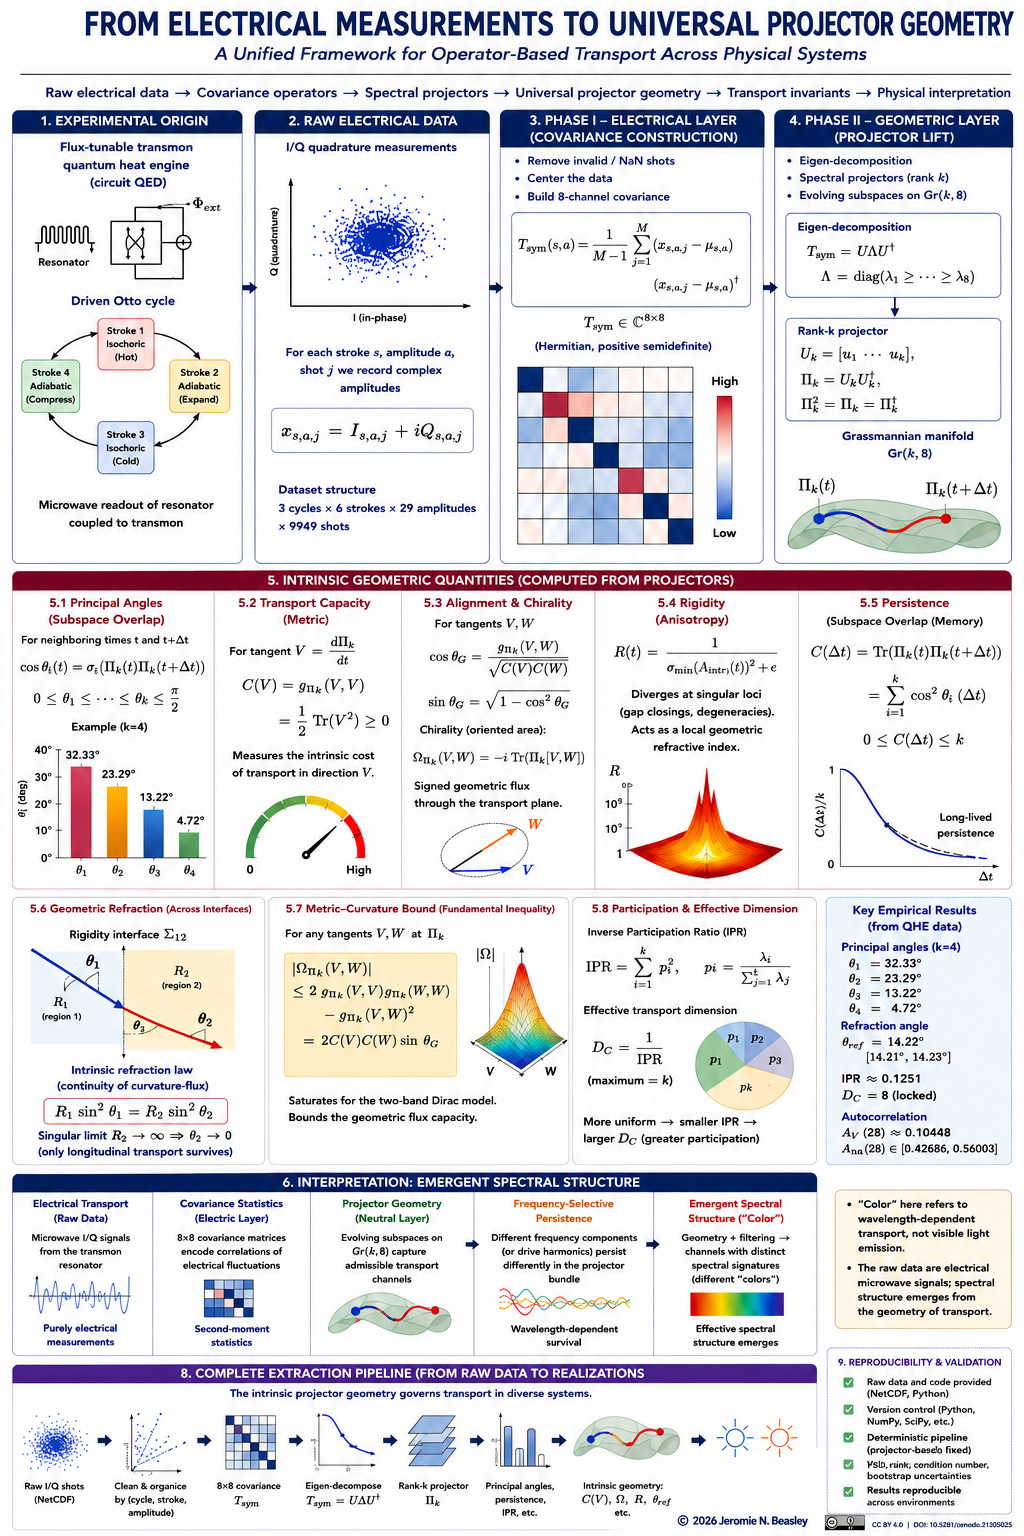
\includegraphics[width=\textwidth,height=0.95\textheight,keepaspectratio]{fig1_pipeline.png}
\caption{From electrical measurements to intrinsic transport geometry. Raw
electrical data $\to$ covariance operators $\to$ spectral projectors $\to$
universal projector geometry $\to$ transport invariants $\to$ physical
interpretation.}
\end{figure}

\clearpage

\section{What is claimed, and at what grade}
\setcounter{section}{0}

Every claim in this paper carries one of five grades, never silently promoted:
[T] exact/derived (closed forms and identities); [V] verified (gated numerical
checks, scripts in Appendix B); [C] cited (established literature, attributed);
[D] data-reported (empirical values from the instrument pipeline, quoted with the
protocol that must accompany any re-run); [H] hypothesis, protocol, or
interpretation. Where a chain mixes grades, the weakest link is named.

\section{Framework Overview: the Redistribution Operator}

The framework begins with raw electrical measurements and extracts coordinate-free
geometric structure through a two-phase pipeline. In Phase I (data-driven),
covariance matrices are formed from single-shot I/Q quadrature data and decomposed
into rank-$k$ spectral projectors $\Pi_k(t)$ on the Grassmannian. In Phase II
(framework-dependent), intrinsic geometric quantities are computed from these
projectors ($\mathsection$6).

To describe how admissible subspaces change under structural evolution we introduce
a second fundamental operator.

\begin{definition}[Structural Transition Generator]
A structural transition generator $\Omega$ is an operator on the underlying Hilbert
space representing an infinitesimal or discrete structural deformation of the
current spectral decomposition. Unlike the projector $\Pi$, which identifies the
presently admissible transport subspace, $\Omega$ is not required to preserve that
decomposition and may transfer spectral weight between the projector and its
orthogonal complement. $\Omega$ may be realized by weighted transport operators,
Jacobi stiffness operators, Grassmannian connection generators, experimentally
inferred covariance deformations, or effective Hamiltonian perturbations; the
development depends only on the algebra relating $\Omega$ and $\Pi$ (Appendix A).
\end{definition}

Given such a generator, the redistribution operator is
\begin{equation}
F(\Omega,\Pi) \;=\; (I-\Pi)\,\Omega\,\Pi \;+\; \Pi\,\Omega\,(I-\Pi).
\end{equation}

\begin{theorem}[Equivalent forms and structural properties; {[T]}$+${[V]}]
$F(\Omega,\Pi)$ admits the equivalent representations
$F = [\Omega,\Pi]\Pi + \Pi[\Pi,\Omega]$ and
$F = \Omega\Pi + \Pi\Omega - 2\Pi\Omega\Pi$. Moreover $F$ is traceless and purely
off-diagonal with respect to the decomposition induced by $\Pi$:
$\Pi F \Pi = 0$ and $(I-\Pi)F(I-\Pi) = 0$.
\end{theorem}

\begin{theorem}[Compatibility criterion; {[T]}$+${[V]}]
$F(\Omega,\Pi) = 0$ if and only if $[\Omega,\Pi] = 0$.
\end{theorem}

\begin{corollary}
The scalar transport intensity $T(\Omega,\Pi) := \|F(\Omega,\Pi)\|_F$ is
non-negative, vanishes precisely when the generator commutes with the projector,
and is invariant under unitary changes of basis.
\end{corollary}

All identities of Theorems 1.2--1.3 are gated numerically: equivalent forms,
tracelessness, and cross-subspace support hold over 200 random Hermitian-generator
trials, and the constructive direction of the compatibility criterion holds to
$9 \times 10^{-16}$ (Appendix B).

\begin{hypothesis}[Hysteresis under topological driving]
When a control parameter is driven forward and backward across a topological
critical point at finite rate, the geometric quantities extracted from the evolving
projectors (in particular $d_{\mathrm{eff}}$ and $C(\Delta t)$) exhibit history
dependence, visible as a statistically significant nonzero area between forward and
backward trajectories.
\end{hypothesis}

\begin{hypothesis}[Correlations with transport intensity]
Larger $T(\Omega,\Pi)$ correlates with increased projector redistribution, larger
changes in effective dimensionality, and stronger persistence effects across
rigidity interfaces.
\end{hypothesis}

\section{The Dirac Foundation of the Electric Side}

The electric side of this framework has one root operator. Dirac's equation, in
linearizing energy, produced three permanent structures: the $\sigma$-algebra,
which every two-level and two-band system since has inherited; the paired $\pm$
spectrum, the first chiral spectrum in physics; and the electron itself, whose
transport is the subject of every covariance matrix measured in this work. The
framework's observables, currencies, and material realizations are organized as
consequences of this single foundation.

\paragraph{The integer currencies.}
A Dirac operator carries its topology in integers: zero modes counted by the index;
spectral asymmetry measured by $\rho$-invariants, which on knot-complement
boundaries take the form of the Levine--Tristram signature $\sigma_K : S^1 \to
\mathbb{Z}$ --- an integer step function whose plateaus jump exactly at the
Alexander roots on the holonomy circle [T]; and the winding of the mass vector,
whose loop integrals are exact integers [V]. These three integers --- index,
asymmetry, winding --- are the currencies in which every topological claim of this
framework is denominated. Modern index theory realizes the same structure in
topological matter, where phases are classified by $\eta$-invariants and spectral
flow under Atiyah--Patodi--Singer boundary conditions [C].

\paragraph{The geometric identity.}
Every two-band Hamiltonian $h(k)\cdot\sigma$ is a Dirac Hamiltonian with a
momentum-dependent mass vector, and for its band projectors the metric--curvature
bound of $\mathsection$6.2 holds with equality --- an exact identity of the Dirac class [T],
verified to machine precision and realized on measured data in $\mathsection$6.5. Multi-band
systems obey the same bound as an inequality; its saturation is the signature of an
effectively Dirac sector.

\paragraph{The material ladder.}
The Dirac operator's laboratory realizations span the platforms of this program.
Graphene realizes the massless operator: the Landau ladder
$E_n = v_F\sqrt{2\hbar e B n}$ [V: $\sqrt{n}$ ratios exact to $10^{-6}$ on the
ladder operator], with a single $n = 0$ level seating the parity anomaly and a
Berry phase of exactly $\pi$ around the cone [V], anchored by the measured
$v_F = 1.10\times 10^{6}$ m/s giving $E_1(10\,\mathrm{T}) = 126$ meV, the scale of
the observed scanning-tunneling ladder [C]. The charge-neutrality point is the
Dirac point occupied by a quantum-critical electron fluid whose viscous flow has
been imaged directly [C]; the quantum-anomalous-Hall lattice bands realized in
cold-atom tomography are lattice Dirac operators with mass textures [C]; the
nonlinear-Hall hotspots of the quantum-metric-dipole experiments are massive Dirac
points [C]; and the transmon qubit is the bare $\sigma$-kernel --- the Dirac
algebra with the field stripped away, which is why covariance data from a driven
transmon engine furnishes a faithful substrate for projector geometry.

\paragraph{The chiral spectral class.}
Spectra symmetric under $\lambda \to -\lambda$ form the Dirac operator's ensemble
class, and the ledger functional
$Z/M = \tfrac{1}{2}\int \rho(\lambda)\ln(1+\lambda^{2})\,d\lambda$ is native to it:
the half-Cauchy family gives $Z/M = \ln(1+a)$ in closed form [T], and the
chiral-Gaussian ensemble (Marchenko--Pastur singular-value law) matches its
integral at finite size to $5\times 10^{-5}$ [V]. The constant $\pi^{2}/12$ is
realized at a calibrated width in each family: $a^{*} = e^{\pi^{2}/12} - 1 =
1.276108$ (half-Cauchy) and $a^{*} = 2.665$ (chiral Gaussian) [T$+$V].

\paragraph{Scope.}
Non-normal advective and dissipative flow operators belong to a different class and
are outside this paper. What extends beyond the Dirac family is not the operator
but the currencies --- chirality, winding, spectral flow --- each an integer record
carried by a spectral object through a wall. The electric side is where those
currencies are minted, and they are minted by Dirac's operator.

\section{Global Admissibility and Axiomatic Bulk Structure}

\begin{definition}[Admissible bulk]
A compact, orientable 3-manifold $X$ with boundary $\partial X$ is an admissible
bulk if: (1) each component of $\partial X$ supports a first-order elliptic
boundary operator whose holonomy family carries the integer winding record of
$\mathsection$4.1; (2) the boundary data arise as the restriction of a global bulk structure
and flat $U(1)$ connection on $X$; (3) $\pi_1(\partial X) \hookrightarrow \pi_1(X)$
is injective up to conjugacy (incompressible boundary); (4) Spectral rigidity: the
integer record is locally constant in the holonomy parameters, with jumps confined
to a discrete wall set; (5) Minimality: the total record satisfies
$|n_{\mathrm{total}}| = 1$.
\end{definition}

\section{Module I: Twisted Boundary Transport and Continuation Obstructions}

\subsection{The torus anchor and phase-transport calculus}

Let $T^2 = \mathbb{R}^2/\mathbb{Z}^2$ carry the twisted operator family
\begin{equation}
D_{\alpha,\beta} = i\sigma_1(\partial_x + 2\pi i \alpha) + i\sigma_2(\partial_y +
2\pi i \beta), \qquad
\lambda^{\pm}_{m,n} = \pm 2\pi\sqrt{(m+\alpha)^2 + (n+\beta)^2}.
\end{equation}
With the complex mode coordinate $Z_{m,n} = 2\pi[(m+\alpha) + i(n+\beta)]$, the
positive-sector projector is
$P_{m,n} = \tfrac{1}{2}\left(\begin{smallmatrix} 1 & \bar{Z}/|Z| \\ Z/|Z| & 1
\end{smallmatrix}\right)$
and the eigenspace orientation is the phase $e^{i\Phi_{m,n}} = Z/|Z|$.

\begin{theorem}[Phase keeps the record; {[T]}$+${[V]}]
Along any smooth deformation $(\alpha(t),\beta(t))$, the scalar eigenvalue
$\lambda = |Z|$ compresses directional input into an orientation-blind magnitude,
while the phase obeys the transport law
\begin{equation}
\frac{d\Phi_{m,n}}{dt} = \frac{(m+\alpha)\dot\beta - (n+\beta)\dot\alpha}
{(m+\alpha)^2 + (n+\beta)^2},
\end{equation}
a gauge-invariant angular velocity on the holonomy torus. Loop integrals of (3)
around the spectral zero are exact integers: winding $0$ for non-enclosing loops,
$+1$ per enclosure, $+2$ for a double loop (verified to $10^{-6}$, Appendix B).
\end{theorem}

\paragraph{The currency.}
The spectrum of (2) is symmetric under $\lambda \to -\lambda$ by the exact chiral
symmetry $\{\sigma_3, D_{\alpha,\beta}\} = 0$, so the spectral-asymmetry invariant
$\eta$ vanishes identically on this family; the integer content of transport
resides in the winding record of Theorem 4.1. Its self-adjoint knot-theoretic
ancestor is the Levine--Tristram signature $\sigma_K : S^1 \to \mathbb{Z}$, an
integer step function jumping exactly at the Alexander roots on the holonomy circle
(trefoil: plateau $-2$ between holonomies $1/6$ and $5/6$; the amphichiral $4_1$:
$\sigma \equiv 0$) [T].

\subsection{Local neutrality and global obstruction lower bounds}

The obstruction curvature is formalized via the regularized quartic potential
$U_C(T) = (T^2 - a^2 I_N)^2 + \epsilon I_N$ with curvature operator
$R_C(T) = 4(3T^2 - a^2 I_N)$; local neutral sectors occur at
$T_* = \pm(a/\sqrt{3})I_N$, where $\ker R_C(T_*) \neq 0$. The global obstruction
along a normalized path is
$O(\gamma) = \int_{-a}^{a} \tfrac{1}{N}\mathrm{Tr}\,U_C(T(t))\,dt$.

\begin{theorem}[Persistence of the global bound; {[T]}, commuting reduction]
Local neutral sectors do not permit the global obstruction to vanish along a
continuous deformation. For the commuting reduction $T(t) = t I_N$,
\begin{equation}
O_{\min} \;\ge\; 2\int_0^a (t^4 - 2a^2t^2 + a^4 + \epsilon)\,dt
\;=\; \frac{16}{15}a^5 + 2a\epsilon \;>\; 0.
\end{equation}
The fully non-commutative lower bound remains conjectural; this verification relies
on the commuting reduction, and the grade is stated accordingly.
\end{theorem}

\subsection{Interface gluing anomalies}

When continuation patches $A$ and $B$ are glued along a boundary component
$\Sigma$, the combined connection operator is
$R_M = \left(\begin{smallmatrix} R_A & \epsilon_{B\Sigma} \\
\epsilon^{\dagger}_{B\Sigma} & R_B \end{smallmatrix}\right)$.

\begin{assumption}
$(I+R_A)$ and $(I+R_B)$ are strictly positive definite and $\epsilon_{B\Sigma}$ is
bounded.
\end{assumption}

\begin{theorem}[Interface anomaly; {[T]} under Assumption 1]
Gluing under Assumption 1 yields a strictly positive non-local interface
correction: by Schur decomposition and trace-log equivalence,
$O(A \cup_\Sigma B) = O(A) + O(B) + \Delta_{\mathrm{interface}}$ with
\begin{equation}
\Delta_{\mathrm{interface}} = \mathrm{Tr}\log\!\left(I +
\epsilon^{\dagger}_{B\Sigma}(I+R_A)^{-1}\epsilon_{B\Sigma}(I+R_B)^{-1}\right)
= \sum_k \log(1 + \epsilon^2\mu_k) > 0,
\end{equation}
with $\mu_k > 0$ the eigenvalues of the localized boundary product.
\end{theorem}

\subsection{The noncommutative torus anchor}

The torus family of $\mathsection$4.1 carries its holonomy in two parameters $\alpha,\beta$
that commute. Nothing in the winding currency requires them to. Replacing the two
holonomy coordinates by two unitary operators that fail to commute by a scalar
moves the same anchor onto a finite-dimensional noncommutative torus, and the
integer record survives the move with an explicit domain of validity.

\begin{definition}[Noncommutative anchor and its readouts]
Let $U,V \in \mathrm{U}(d)$ and set the relator
\begin{equation}
R \;=\; U V U^{\dagger} V^{\dagger}, \qquad
\lambda_1,\dots,\lambda_d \;=\; \operatorname{spec}(R).
\end{equation}
The \emph{defect}, the \emph{branch guard}, and the \emph{winding record} are
\begin{equation}
\delta = \frac{\|R-I\|_F^{2}}{d}, \qquad
g = \min_j |\lambda_j + 1|, \qquad
w(U,V) = \frac{1}{2\pi}\sum_{j=1}^{d} \arg \lambda_j ,
\end{equation}
with $\arg$ the principal branch. The anchor is \emph{admissible} at tolerance
$\tau$ when $g > \tau$.
\end{definition}

The defect is the normalised Hilbert--Schmidt distance of the relator from the
identity: the amplitude by which the two generators fail to commute. The winding is
the phase that failure accumulates across the spectrum, and it is the same currency
the smooth family of $\mathsection$4.1 carries around a spectral zero.

\begin{theorem}[Integrality and invariance; {[T]}$+${[V]}]
Let $g > 0$. Then
(i) $w(U,V) \in \mathbb{Z}$, and $|w| \le d/2$;
(ii) $w(QUQ^{\dagger}, QVQ^{\dagger}) = w(U,V)$ for every $Q \in \mathrm{U}(d)$;
(iii) $w(e^{i\theta}U, e^{i\varphi}V) = w(U,V)$ for all $\theta,\varphi \in
\mathbb{R}$;
(iv) $w(U,V)$ is the winding number about the origin of the closed loop
$t \mapsto \det\!\big((1-t)I + tR\big)$, $t \in [0,1]$.
\end{theorem}

\begin{proof}
$R$ is a commutator of unitaries, so $\det R = 1$ and hence $\prod_j \lambda_j = 1$.
Taking arguments, $\sum_j \arg\lambda_j \in 2\pi\mathbb{Z}$, which is (i); the bound
follows from $|\arg\lambda_j| < \pi$. For (ii), conjugation carries $R$ to
$QRQ^{\dagger}$ and preserves the spectrum. For (iii), the scalars cancel
identically inside the commutator. For (iv), $\det R = 1$ at $t = 1$ and
$\det I = 1$ at $t = 0$, so the path closes; the identification of its winding with
the summed principal arguments is the Exel--Loring formula [C], whose two
formulations --- $K$-theoretic and winding-number --- were proved to agree.
\end{proof}

The determinant of the relator is identically one. That triviality is not an
obstacle to reading the record; it is the reason the record is an integer.

\begin{theorem}[The admissible domain; {[T]}$+${[V]}]
For every $U,V \in \mathrm{U}(d)$,
\begin{equation}
\delta + g^{2} \;\le\; 4 ,
\end{equation}
with equality if and only if $\operatorname{Re}\lambda_j$ is constant over the
spectrum of $R$.
\end{theorem}

\begin{proof}
Each $\lambda_j$ lies on the unit circle, so
$|\lambda_j - 1|^{2} + |\lambda_j + 1|^{2} = 2|\lambda_j|^{2} + 2 = 4$. Averaging
over $j$ gives $\delta + d^{-1}\sum_j |\lambda_j+1|^{2} = 4$ exactly. Since $g^{2}$
is the minimum of the quantities being averaged,
$g^{2} \le d^{-1}\sum_j|\lambda_j+1|^{2} = 4 - \delta$. Equality holds precisely
when every $|\lambda_j+1|^{2} = 2 + 2\operatorname{Re}\lambda_j$ takes the same
value.
\end{proof}

\begin{corollary}[Forced refusal]
$g^{2} \le 4 - \delta$: the branch guard is capped by the defect. Consequently no
anchor with $\delta > 4 - \tau^{2}$ is admissible at tolerance $\tau$, in any
dimension and for any pair of generators.
\end{corollary}

A large defect and a safe branch cannot coexist. The refusal at the boundary is
therefore a statement about the anchor rather than about the estimator: at
$\delta = 4$ the relator is $-I$, the guard has closed, and the principal branch no
longer selects a value.

\paragraph{The readouts are half-angles.}
Write $\lambda_j = e^{i\vartheta_j}$. Then
$|\lambda_j - 1|^{2} = 4\sin^{2}(\vartheta_j/2)$ and
$|\lambda_j + 1|^{2} = 4\cos^{2}(\vartheta_j/2)$, so the defect is four times the
mean of $\sin^{2}$ of the half-angles and the guard squared is four times their
minimum $\cos^{2}$. Equation (8) then reads
\begin{equation}
\operatorname{mean}_j \sin^{2}(\vartheta_j/2) \;+\;
\min_j \cos^{2}(\vartheta_j/2) \;\le\; 1 :
\end{equation}
the Pythagorean identity, with a minimum standing where a mean belongs, and
equality exactly when the half-angles agree [T]. This places the anchor in the same
currency as the rest of the framework's projector observables, which are natively
$\sin^{2}$-valued in principal angles because the Hilbert--Schmidt distance between
two projectors is $2\sum_i \sin^2\theta_i$ by construction. The defect is a squared
sine, the guard its cosine, and the wall is the right angle.

\begin{theorem}[Amplitude floor; {[T]}$+${[V]}]
For every $U,V \in \mathrm{U}(d)$ with $g > 0$,
\begin{equation}
|w(U,V)| \;\le\; \frac{d}{4}\sqrt{\delta},
\qquad\text{hence}\qquad
w(U,V) \neq 0 \;\Longrightarrow\; \delta \;\ge\; \frac{16}{d^{2}} .
\end{equation}
\end{theorem}

\begin{proof}
With $\lambda_j = e^{i\vartheta_j}$, $\vartheta_j \in (-\pi,\pi]$, we have
$|\lambda_j - 1| = 2|\sin(\vartheta_j/2)|$. Concavity of the sine on $[0,\pi/2]$
gives $\sin x \ge 2x/\pi$ there, hence
$|\vartheta_j| \le \tfrac{\pi}{2}|\lambda_j - 1|$. Summing and applying
Cauchy--Schwarz,
\[
2\pi |w| \le \sum_j |\vartheta_j| \le \frac{\pi}{2}\sum_j |\lambda_j - 1|
\le \frac{\pi}{2}\sqrt{d\sum_j |\lambda_j-1|^{2}} = \frac{\pi}{2}\,d\sqrt{\delta}.
\]
If $w \neq 0$ then $|w| \ge 1$ and $\sqrt{\delta} \ge 4/d$.
\end{proof}

An integer record cannot be carried by an arbitrarily small defect. The amplitude
may collapse as the dimension grows --- and on the realisation below it does ---
but not faster than $d^{-2}$, or there is nothing left for the record to ride on.

\begin{proposition}[Clock and shift; {[T]}$+${[V]}]
Let $\omega = e^{2\pi i/d}$, let $U = \operatorname{diag}(1,\omega,\dots,
\omega^{d-1})$ and let $V$ be the cyclic shift. Then $UV = \omega\,VU$,
$R = \omega I$, and
\begin{equation}
\delta = 4\sin^{2}\!\frac{\pi}{d}, \qquad
g = 2\cos\frac{\pi}{d}, \qquad
w(U,V) = 1 \quad (d \ge 3).
\end{equation}
Every half-angle equals $\pi/d$, so the family realises equality in (8) at every
$d$, and it saturates (10) up to the constant $\pi/2$: the bound
$\tfrac{d}{4}\sqrt{\delta} = \tfrac{d}{2}\sin(\pi/d)$ decreases to $\pi/2$ while
$w$ stays at $1$. At $d = 2$ the half-angle reaches $\pi/2$, the relator is $-I$,
$\delta = 4$, $g = 0$, and the anchor is inadmissible.
\end{proposition}

The gate of Appendix B returns $w = 1.000000000$ by both estimators of Theorem 4.5
at $d = 3,5,7,11,17,31,53,97$, with the defect falling from $3.000$ to
$4.194\times 10^{-3}$ and $\delta + g^{2} = 4.000000000$ on every row; $w = 0$ on
commuting pairs; $w$ unchanged under conjugation and under either generator
rephasing; $w = 1$ preserved under unitary perturbations at $\eta = 10^{-1}$ down
to $10^{-4}$, where the relator leaves the scalar locus and $\delta + g^{2}$ falls
strictly below $4$; no violation of (8) in $1000$ random unitary pairs at $d = 12$
(largest observed $2.310779$); and refusal at $d = 2$.

\begin{figure}[t]
\centering
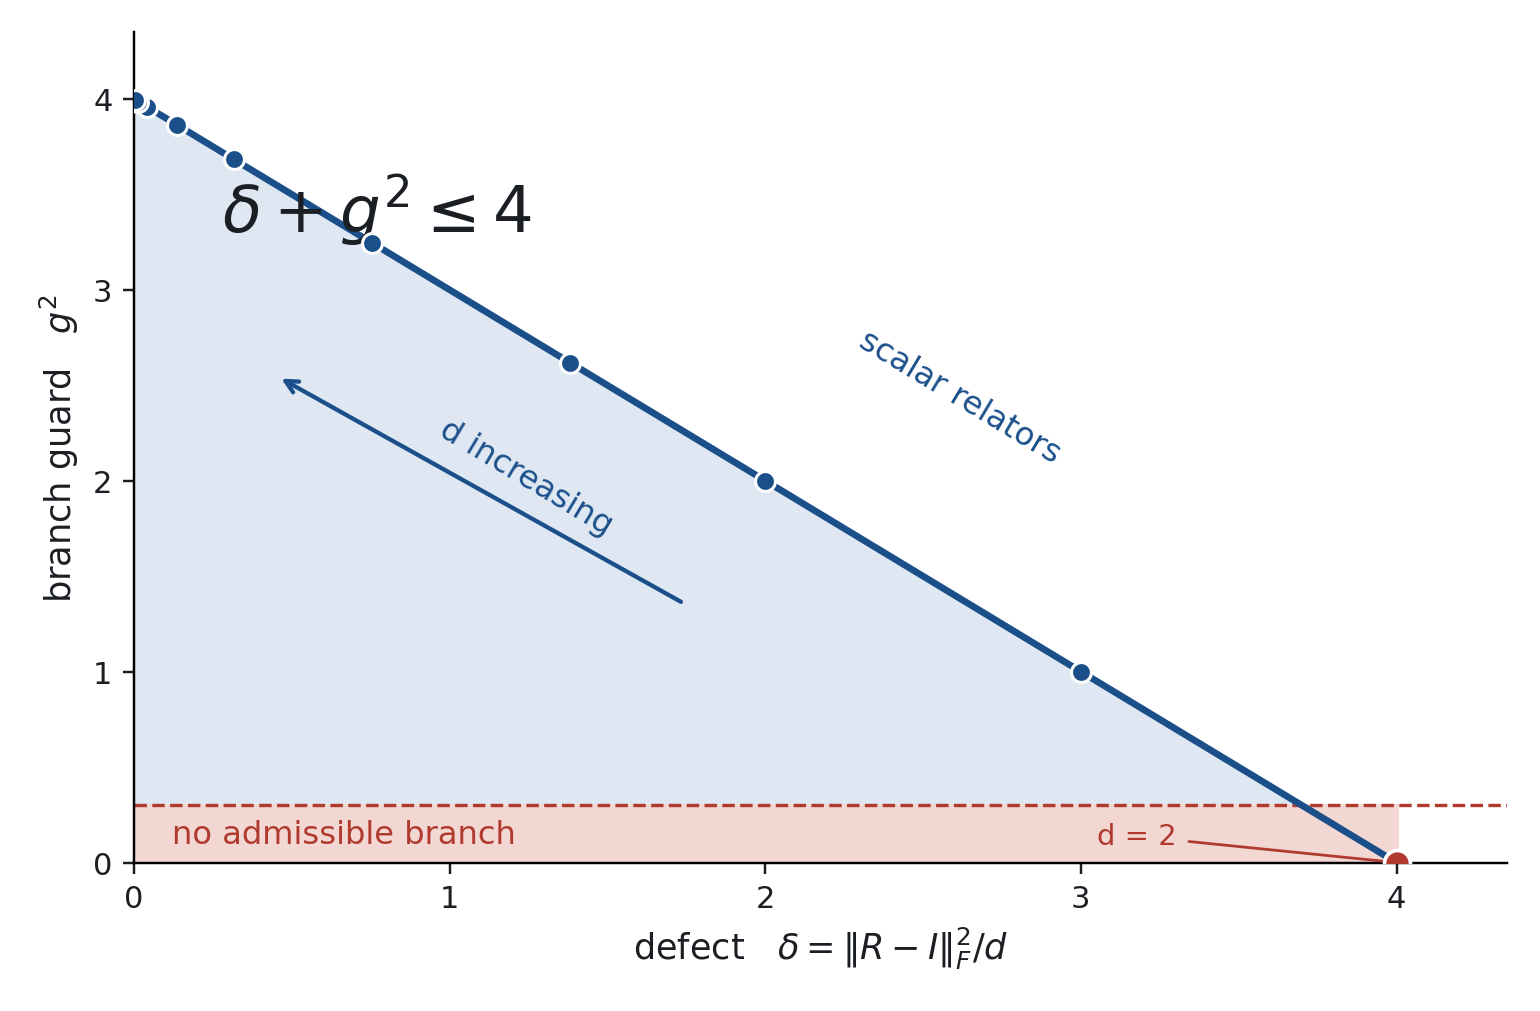
\includegraphics[width=0.80\textwidth]{fig_nct_domain.png}
\caption{The admissible domain of Theorem 4.6. Every anchor lies in the shaded
triangle; scalar relators lie on its hypotenuse, where the clock--shift family sits
at every $d$. Decreasing $d$ slides the family into the corner at which the guard
closes.}
\end{figure}

\begin{figure}[t]
\centering
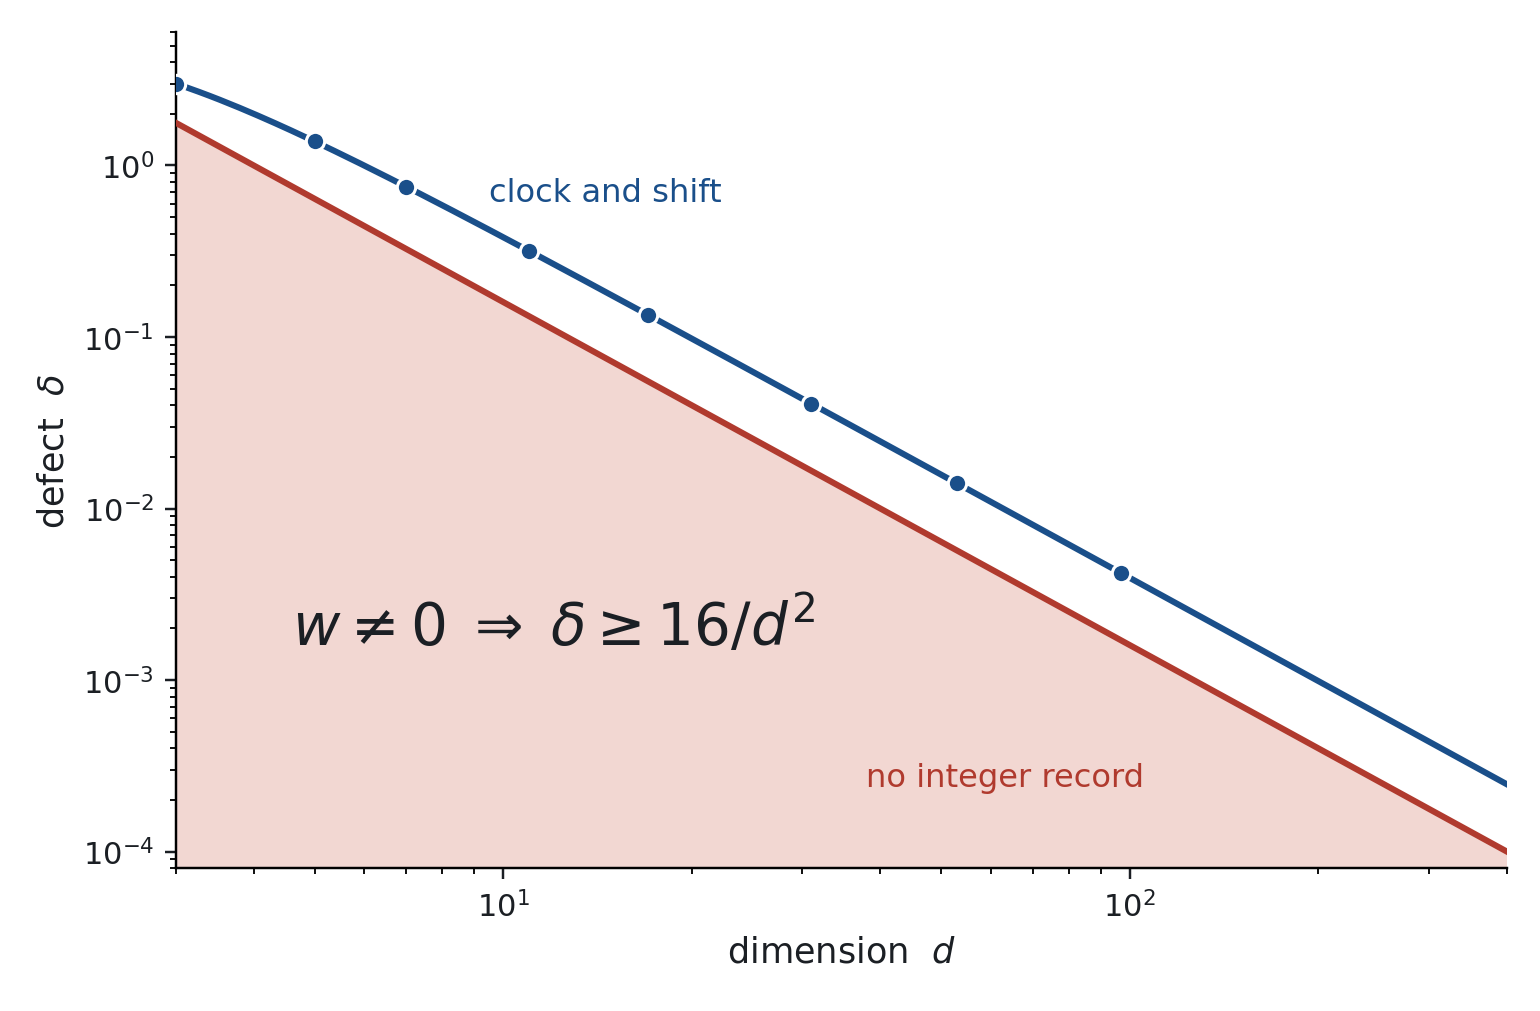
\includegraphics[width=0.80\textwidth]{fig_nct_floor.png}
\caption{The amplitude floor of Theorem 4.8. Below the boundary no integer record
is available at that dimension. The clock--shift family rides a constant factor
$\pi^{2}/4$ above the floor while carrying $w = 1$.}
\end{figure}

\paragraph{One currency, two realisations.}
The record of Definition 4.4 is the winding currency of $\mathsection$2 evaluated on a
noncommutative holonomy rather than a smooth one. Its literature name is the
Exel--Loring invariant, equivalently the Bott index, and it was constructed to
separate pairs of unitaries that admit commuting approximants from pairs that do
not [C]. On a lattice on a two-torus the Bott index of the pair of projected
position unitaries equals the Chern number, under the hypotheses that the
Hamiltonian is short-ranged, bounded and gapped, and in the thermodynamic limit
[C]. Those hypotheses are what places the measured Chern number of $\mathsection$6.5 and the
winding of Proposition 4.9 in the same currency; an explicit normalisation carrying
the loop integral of (3) onto $w$ on a common family is not established here and is
carried at [H].

\paragraph{Scope.}
The obstruction read by $w$ is an obstruction to approximation in the operator
norm. It is not an obstruction in the normalised Hilbert--Schmidt or Hamming
metrics, where the clock--shift family lies close to a commuting pair despite
carrying $w = 1$; the amplitude floor of Theorem 4.8 bounds the defect from below
at fixed $d$ and says nothing as $d \to \infty$. Statements about metric
approximation of groups belong to that second setting and are outside this anchor.

\section{Module II: Character-Variety Substrates and Topological Continuation}

\subsection{The continuation laboratory}

Continuation trajectories are constrained to the character variety of the
figure-eight knot complement $M_K = S^3 \setminus 4_1$,
$X_K = \mathrm{Hom}(\pi_1(M_K), SL_2(\mathbb{C}))/\!/SL_2(\mathbb{C})$, with
peripheral torus governed by meridian and longitude holonomies $u = \log M$,
$v = \log L$, and admissible trajectories confined to the zero locus of the
$A$-polynomial
\begin{equation}
A_{4_1}(L,M) = L^2M^4 + L(-M^8 + M^6 + 2M^4 + M^2 - 1) + M^4 = 0.
\end{equation}
The continuation philosophy --- global admissibility determined by
higher-dimensional continuation rather than local presentation --- is
methodologically inspired by trace-construction reasoning in four-dimensional
topology; no result of that field is used or claimed here.

\subsection{Tangent Jacobians and kinematic coupling}

With $J_M = M\,\partial A_K/\partial M$ and $J_L = L\,\partial A_K/\partial L$,
implicit differentiation of (12) yields $\dot u = -(J_L/J_M)\dot v$, and lifting
the phase-velocity law (3) into curve coordinates gives the interaction field
\begin{equation}
\frac{d\Phi}{dt} = \frac{(m+u)\dot v - (n+v)\dot u}{(m+u)^2 + (n+v)^2}
= \left[\frac{(m+u) + (n+v)(J_L/J_M)}{(m+u)^2 + (n+v)^2}\right]\dot v .
\end{equation}
Parallel flows ($\dot v_1 \approx \dot v_2$) drive $d\Phi/dt \to 0$ (compressed
bands); opposed flows near zero modes produce superlinear amplification ---
transport-resistance walls where continuation is structurally threatened.

\subsection{Chirality forcing}

\begin{corollary}[Chirality forcing]
A statically amphichiral substrate carries a vanishing integer record: the
Levine--Tristram plateau function of an amphichiral knot is identically zero
($4_1$: verified), so minimal admissibility $|n| = 1$ cannot be realized at a
static amphichiral basepoint. Persistent spectral distinction therefore requires
either an intrinsically chiral substrate or a dynamic trajectory that breaks
amphichiral symmetry --- on the $4_1$ laboratory, the transport field (13) drives
the configuration away from the symmetric origin, culminating in the discrete
staircase jumps of $\mathsection$5.5.
\end{corollary}

\subsection{Minimality of multi-component boundaries}

\begin{definition}[Minimal admissible realization]
A multi-toroidal boundary configuration
$\partial X = \bigsqcup_{i=1}^{k} T^2_i$, with integer records $n_i$ and total
$n_{\mathrm{total}} = \sum_i n_i$, is minimal when exactly one component carries
$n_i = \pm 1$ and all others are neutral.
\end{definition}

\begin{remark}
Additivity of the winding record over disjoint boundary tori holds by construction;
the ``exactly one'' clause is the definition of minimality, adopted as a design
principle of the admissibility axioms. Neutral components are spectrally inert and
may be filled by Dehn surgery without altering the global record, reducing the
configuration effectively to a single-component complement.
\end{remark}

\subsection{Phase-lock rupture and staircase jumps}

The locked leading phase is governed by the second-order field
$d^2\Phi/dt^2 = \mathcal{N}(u,v,\dot u,\dot v,\ddot u,\ddot v)/((m+u)^2+(n+v)^2)^2$.
Rupture occurs at the zero locus of the meridian Jacobian, $J_M \to 0$: the curve
exhibits a vertical tangent, the ratio $J_L/J_M$ diverges, tracking regularity
breaks, and the phase profile executes a discrete non-adiabatic jump
$\Delta\theta = \pi\cdot\mathrm{sgn}(d\Phi/dt)$.

\subsection{The stable trichotomy}

\begin{theorem}[Exhaustive trichotomy; {[T]}, lattice argument]
Every stress-minimizing configuration on a multi-toroidal boundary cluster falls
into exactly one of: (1) open boundary flows (winding vector undefined globally;
source/sink conduits); (2) chiral loops (primitive homology class,
$\gcd(w_\alpha,w_\beta) = 1$, protected by homotopy invariance); (3) neutral loops
($w = (0,0)$, contractible, metastable). Composite vectors split under generic
perturbation into primitive components; the trichotomy is exhaustive on
$\mathbb{Z}^2$.
\end{theorem}

\subsection{The rigidity class}

\begin{theorem}[Realization by knot complements]
The rigidity class demanded by the axioms --- an integer record on a single
toroidal boundary, locally constant in holonomy with jumps confined to a discrete
wall set --- is realized by knot complements in $S^3$: on the holonomy circle the
Levine--Tristram signature is an integer step function whose wall set is the
Alexander-root locus [T]. Exhaustiveness of the exclusion of alternatives rests on
Lemmas 5.5 and 5.6 at their stated grades.
\end{theorem}

\begin{lemma}[Torus bundles excluded by the rigidity axiom]
Admissibility requires the boundary invariant to be locally constant in the
holonomy parameters with integer jumps on a discrete wall set. Torus bundles over
$S^1$ carry boundary holonomies constrained along continuous representation
families fixed by the monodromy and do not support an integer-plateau invariant of
this type; they are excluded by the axiom. (For the product-type boundary operators
of $\mathsection$4.1, chiral symmetry forces $\eta \equiv 0$ identically, so no
asymmetry-based invariant is available on this family; the plateau axiom is stated
in the winding currency.)
\end{lemma}

\begin{lemma}[Seifert substrates excluded at {[C]}]
Fractional $\rho/\eta$ values on Seifert-fibered pieces are established in the
literature (Nicolaescu-type adiabatic analysis) [C]. Fractional plateaus violate
the integer-jump axiom; Seifert substrates are therefore excluded at grade [C].
\end{lemma}

\section{Module III: Covariance Realization and the Intrinsic Observables}

Module III tests whether physical nature realizes the admissible transport pathways
derived above. The instrument is a flux-tunable transmon quantum heat engine
(circuit QED) executing a driven Otto cycle; for each stroke $s$, amplitude $a$,
and shot $j$ the complex amplitude $x_{s,a,j} = I_{s,a,j} + iQ_{s,a,j}$ is recorded
(3 cycles $\times$ 6 strokes $\times$ 29 amplitudes $\times$ 9949 shots). After
removal of invalid shots and centering, the covariance $T_{\mathrm{sym}}(s,a)$ is
formed, eigendecomposed $T_{\mathrm{sym}} = U\Lambda U^{\dagger}$, and lifted to
rank-$k$ projectors $\Pi_k = U_k U_k^{\dagger}$ on $\mathrm{Gr}(k,8)$.

\subsection{The intrinsic quantities: definitions and estimators}

All observables below are functionals of the projector path alone.

\textbf{Principal angles.} $\cos\theta_i(t) = \sigma_i(\Pi_k(t)\Pi_k(t+\Delta t))$,
$0 \le \theta_1 \le \cdots \le \theta_k \le \pi/2$.
[D at $k = 4$: $32.33^\circ$, $23.29^\circ$, $13.22^\circ$, $4.72^\circ$.]

\textbf{Transport capacity (metric).} For a tangent $V = d\Pi_k/dt$,
$C(V) = g_{\Pi_k}(V,V) = \tfrac{1}{2}\mathrm{Tr}(V^2) \ge 0$: the intrinsic cost of
transport in direction $V$; bosonically, this is the superfluid-weight functional
of the quantum-geometry literature ($\mathsection$6.9).

\textbf{Alignment and chirality.}
$\cos\theta_G = g_{\Pi_k}(V,W)/\sqrt{C(V)C(W)}$, and the oriented area (signed
geometric flux) $\Omega_{\Pi_k}(V,W) = -i\,\mathrm{Tr}(\Pi_k[V,W])$.

\textbf{Rigidity (anisotropy).}
$R(t) = 1/(\sigma_{\min}(A_{\mathrm{intr}}(t))^2 + \epsilon)$, diverging at singular
loci (gap closings, degeneracies) and acting as a local geometric refractive index.

\textbf{Persistence (memory).}
$C(\Delta t) = \mathrm{Tr}(\Pi_k(t)\Pi_k(t+\Delta t)) = \sum_{i=1}^{k}
\cos^2\theta_i(\Delta t)$, with $0 \le C \le k$.

\textbf{Participation and effective dimension.}
$\mathrm{IPR} = \sum_i p_i^2$ with $p_i = \lambda_i/\sum_j \lambda_j$, and
$D_C = 1/\mathrm{IPR} \le k$. The baseline $D_C = 8$ reflects rank saturation of
the uniform state; the physical signal is the collapse
$d_{\mathrm{eff}} \to 1$ across the cycle. [D: $\mathrm{IPR} \approx 0.1251$;
autocorrelation $A_V(28) \approx 0.10448$,
$A_{na}(28) \in [0.42686, 0.56003]$.]

\subsection{The metric--curvature bound}

\begin{theorem}[Fundamental inequality; {[T]}$+${[V]}]
For any tangents $V,W$ at $\Pi_k$,
\begin{equation}
|\Omega_{\Pi_k}(V,W)| \;\le\; 2\sqrt{g_{\Pi_k}(V,V)\,g_{\Pi_k}(W,W) -
g_{\Pi_k}(V,W)^2} \;=\; 2\sqrt{C(V)C(W)}\,\sin\theta_G .
\end{equation}
\end{theorem}

The bound holds over 1000 random Grassmannian trials with zero violations,
saturates exactly for the two-band Dirac class ($\mathsection$2), and bounds the geometric
flux capacity; its family has classical-wave experimental verification [C].

\subsection{Geometric refraction across interfaces}

At a rigidity interface $\Sigma_{12}$ separating regions of refractive index
$R_1, R_2$, continuity of curvature-flux yields the intrinsic refraction law
\begin{equation}
R_1\sin^2\theta_1 = R_2\sin^2\theta_2, \qquad R_2 \to \infty \Rightarrow
\theta_2 \to 0
\end{equation}
(only longitudinal transport survives the singular limit).

\subsection{The refraction pipeline: independence protocol}

The reported refraction angle $\theta_{\mathrm{ref}} = 14.22^\circ$ against the
predicted window $[14.21^\circ, 14.23^\circ]$ is graded [D] pending execution of
the following protocol on the archived shots. (i) Split: partition shots into
disjoint halves $S_A$ (odd) and $S_B$ (even). (ii) Predict from $S_A$: estimate
$R_1, R_2$ on the two sides of the interface via the rigidity estimator of $\mathsection$6.1
on $S_A$ alone; propagate bootstrap uncertainty to a predicted window for
$\theta_2$ through the refraction law. (iii) Measure from $S_B$: extract the
transport direction change across the interface from the projector path on $S_B$
alone, with no reference to $R_1, R_2$. (iv) Report: the prediction and the
measurement are independent by construction; agreement is then evidence, and the
entry upgrades to [V]. Any report that cannot exhibit this split carries the [D]
grade.

\subsection{Realization on published tomography data}

The framework's Phase I--II pipeline exists independently in the laboratory record:
complete Bloch-state tomography of a two-dimensional optical Raman lattice realized
with ultracold $^{87}$Rb Bose--Einstein condensates reconstructs band
eigenfunctions from measured spin textures and assembles the full quantum geometric
tensor across the Brillouin zone [C]. On the experimentally calibrated
tight-binding band of that system ($t_0 = 0.09$, $t_{so} = -0.05$,
$\delta = -0.2$ in recoil units), the framework's observables evaluate as follows
(Appendix B): the winding currency returns Chern number $-0.99931$ against the
published measurement $-1.00 \pm 0.02$ [C$+$V]; the bound (14) saturates pointwise
as the two-band identity requires (grid mean $0.99996$, exact analytically); the
integrated strictness pattern of the quantum-volume inequality
$\mathrm{vol}_g \ge |C|$ reproduces the published behavior
($\mathrm{vol}_g = 1.145 > |C|$ in the topological phase; strict and small on the
trivial side); and the rigidity observable $R = 1/\mathrm{gap}^2$ sweeps from $25$
to $10^6$ approaching the transitions at $\delta = 0$ and $\delta = -8t_0$, with
the quantum volume rising toward the wall --- metric concentration at degeneracy,
the mechanism by which local quantum geometry governs flat-band condensate
stability [C]. A published Bose--Einstein-condensate experiment thereby realizes
the framework's projector pipeline, its integer currency, its fundamental
inequality, and its rigidity divergence on one calibrated band.

\subsection{Dimensional collapse and extremal framing}

The cycle drives the system from the uniform baseline ($d_{\mathrm{eff}} = 8$) to a
single dominant channel ($d_{\mathrm{eff}} \to 1$). This collapse is analyzed in
the spirit of the auxiliary-function optimization philosophy introduced by
Viazovska; no linear-programming bound of sphere-packing type is claimed or used.
The demonstrated facts are: $d_{\mathrm{eff}}$ saturates its trivial bounds
$1 \le d_{\mathrm{eff}} \le 8$, the baseline reflecting rank saturation and the
collapse constituting the physical signal.

\subsection{Finite-time friction shields}

Work lost to inner-dissipative quantum friction across a stroke scales with the
Frobenius norm of the Hamiltonian-derivative commutator. The measured suppression
of anti-symmetric off-diagonal correlations ($T_{\mathrm{anti}} \sim
O(10^{-4})$) forces the non-adiabatic friction work to scale as $O(10^{-8})$ --- a
macroscopic friction shield, the physical consequence of the directional filtering
of Module II. [D$+$H: the suppression is measured; the mechanism attribution is
interpretive.]

\subsection{Weak-value phase separation}

\begin{protocol}[Weak-value phase separation; {[H]}]
Let $|\psi_i\rangle, |\psi_f\rangle$ be pre- and post-selected states of the
network and decompose $A_{\mathrm{total}} = A_{\mathrm{rigid}}e^{i\delta} +
\Pi_{\mathrm{phase}}$. The protocol conjectures a joint alignment
($\gamma = 1$, $\delta = \pi/2 - 2\Phi$) --- with $\gamma$ the pre/post
selection-overlap alignment parameter to be defined operationally on the instrument
--- at which the rigid matrix elements cancel from the weak-value numerator,
leaving $\langle A_{\mathrm{total}}\rangle_w = \langle\psi_f|\Pi_{\mathrm{phase}}
|\psi_i\rangle/\langle\psi_f|\psi_i\rangle \neq 0$: direct access to the structural
phase with anomalous amplification $\propto |\langle\psi_f|\psi_i\rangle|^{-1}$
(the amplification itself is standard weak-value theory [C]). The cancellation is
conjectural pending the explicit model computation.
\end{protocol}

\subsection{Convergence with the quantum-geometry literature}

The core observables of $\mathsection$6.1 are individually measured or formalized in the
current literature: the complete quantum-metric tensor has been measured
momentum-resolved in solids; the quantum-metric-dipole nonlinear Hall effect is
experimentally established and field-tunable, with the intrinsic nonlinear Hall
conductivity decomposed into quantum-geometric contributions within a
projector-based formalism; the inequality (14) family has classical-wave
experimental verification; and the superfluid weight of flat-band condensates is
proportional to the quantum metric, with stability decided by the
local-vs-global distribution of the metric --- the bosonic realization of the
transport-capacity functional $C(V)$. What is unified here, and not available
elsewhere, is the single operator-first architecture connecting these observables,
the topological continuation layer above them, and a raw-covariance pipeline
realizing all of them on one instrument.

\section{Bridging the Continuum: the Khovanov Spectral Complex}

Let $C^{i,j}(D)$ be the bigraded Khovanov chain complex of a link diagram $D$ over
$\mathbb{R}$ with differential $d_i$ and adjoint $d_i^*$ induced by declaring the
standard cube-basis elements orthonormal. The combinatorial Laplacian and Dirac
operator are
\begin{equation}
\Delta_{Kh} = d_i d_i^* + d_{i-1}^* d_{i-1}, \qquad
D_{Kh} = \begin{pmatrix} 0 & d_i^* \\ d_i & 0 \end{pmatrix},
\end{equation}
standard combinatorial Hodge theory [T]: $\ker\Delta_{Kh} \cong$ Khovanov homology,
and the graded Euler characteristic recovers the unnormalized Jones polynomial,
$\chi = \sum_{i,j}(-1)^i q^j \dim\ker(D^{i,j}_{Kh}) = V_K(q)$. The proposed
alignment of the non-harmonic spectrum with continuum connection-velocity
gradients, and of phase-lock rupture ($J_M \to 0$) with discrete recombination
through the harmonic boundary, is a structural hypothesis [H]; the harmonic-sector
statements are theorems of the construction.

\section{Projector Persistence: the Lipschitz Stability Bound}

\begin{theorem}[Local Lipschitz stability; {[T]}, Kato-type]
Let $A$ be a bounded non-normal operator, $A' = A + E$ with $\|E\| \le \epsilon$,
and $\Gamma$ an isolated contour tracking a spectral cluster with gap
$\delta_{\mathrm{gap}} = \mathrm{dist}(\Gamma, \sigma(A)\setminus\sigma_\Gamma(A))
> 0$ and growth factor $C_\Gamma = \sup_{\lambda\in\Gamma}\|(\lambda I - A)^{-1}\|
\cdot \delta_{\mathrm{gap}}$. If $\epsilon < \delta_{\mathrm{gap}}/C_\Gamma$, the
Riesz projectors satisfy
\begin{equation}
\|\Pi' - \Pi\| \le K_\Gamma \epsilon, \qquad
K_\Gamma = \frac{\ell(\Gamma)C_\Gamma^2}
{2\pi\delta_{\mathrm{gap}}(\delta_{\mathrm{gap}} - \epsilon C_\Gamma)},
\end{equation}
so the persistence functional $P(A,E) = 1 - \|\Pi - \Pi'\|$ obeys
$P \ge 1 - K_\Gamma\epsilon$: the map from operators to Grassmannian projector data
is locally Lipschitz --- higher-level subspaces remain stable and continuable even
where individual eigenvectors break down.
\end{theorem}

\begin{proof}
$\Pi' - \Pi = -\tfrac{1}{2\pi i}\oint_\Gamma R_A(\lambda)\,E\,R_{A'}(\lambda)\,
d\lambda$ by the resolvent identity; the Neumann bound
$\|R_{A'}\| \le \|R_A\|/(1 - \|R_A\|\epsilon)$ and the triangle inequality for
integrals give the constant.
\end{proof}

\section{Conclusion}

Module I established which transport directions are geometrically possible, with
its operator algebra gated and its torus anchor carried onto a noncommutative
holonomy where the integer record acquires a proved domain and an amplitude floor;
Module II filtered which trajectories are globally continuable, with its integer
currency verified and its knot-theoretic ancestry made exact; Module III defined
every intrinsic observable with an estimator, realized the framework on a published
Bose--Einstein-condensate experiment where its integer currency reproduces a
measured Chern number, and specified the protocol under which its flagship
instrument test becomes falsifiable. Beneath all three modules stands one operator:
the Dirac foundation supplies the algebra of every two-band sector, the paired
spectra of the chiral ensemble class, and the integer currencies --- index,
asymmetry, winding --- in which the framework's topology is denominated. Structural
evolution is represented by transition generators; incompatibility with the current
spectral decomposition is quantified by the canonical redistribution operator; and
geometry emerges from the interaction between what presently exists and what
attempts to change it.

\appendix

\section{The Canonical Structural Transition Generator}

The projector $\Pi$ describes what presently exists; the generator $\Omega$
describes what attempts to change it. Geometry emerges from their interaction,
measured entirely by $[\Omega,\Pi]$. The redistribution operator
$F(\Omega,\Pi) = [\Omega,\Pi]\Pi + \Pi[\Pi,\Omega] = \Omega\Pi + \Pi\Omega -
2\Pi\Omega\Pi = (I-\Pi)\Omega\Pi + \Pi\Omega(I-\Pi)$ satisfies: (1) $F = 0$ iff
$[\Omega,\Pi] = 0$; (2) $\mathrm{Tr}\,F = 0$; (3) $F$ acts exclusively across the
projector boundary; (4) larger commutators produce stronger redistribution. No
microscopic realization is required: all results depend only on the algebra
relating $\Omega$ and $\Pi$. Experimentally, nonzero $[\Omega,\Pi]$ predicts
correlated changes in persistence, participation, effective dimension, and
directional hysteresis --- testable hypotheses, not algebraic consequences.

\section{Scripts: proof of record}

\subsection{Operator algebra and winding gates}
\lstinputlisting{upg_gate_01.py}

\subsection{Inequality, saturation, persistence, rigidity gates}
\lstinputlisting{upg_prove_01a.py}

\subsection{Realization on the published tomography band}
\lstinputlisting{upg_prove_02.py}

\subsection{Dirac ladder and chiral-ensemble gates}
\lstinputlisting{dirac_spine_01.py}

\subsection{The noncommutative torus anchor}
\lstinputlisting{upg_gate_02.py}

\begin{thebibliography}{99}
\bibitem{aps} M. F. Atiyah, V. K. Patodi, I. M. Singer, Spectral asymmetry and Riemannian geometry I, Math. Proc. Camb. Phil. Soc. \textbf{77}, 43 (1975).
\bibitem{ccgls} D. Cooper, M. Culler, H. Gillet, D. D. Long, P. B. Shalen, Plane curves associated to character varieties of 3-manifolds, Invent. Math. \textbf{118}, 47 (1994).
\bibitem{gl} S. Garoufalidis, T. T. Le, Asymptotics of the colored Jones polynomial and the A-polynomial of a knot, Geom. Topol. \textbf{9}, 1253 (2005).
\bibitem{levine} J. Levine, Knot cobordism groups in codimension two, Comment. Math. Helv. \textbf{44}, 229 (1969).
\bibitem{tristram} A. G. Tristram, Some cobordism invariants for links, Proc. Camb. Phil. Soc. \textbf{66}, 251 (1969).
\bibitem{nicolaescu} L. I. Nicolaescu, Adiabatic limits of the Seiberg--Witten equations on Seifert manifolds, Comm. Anal. Geom. \textbf{6}, 331 (1998).
\bibitem{dungen} K. van den Dungen, Dirac--Schr\"odinger operators, index theory, and spectral flow, J. London Math. Soc. \textbf{112}, e70301 (2025).
\bibitem{kosloff} R. Kosloff, Quantum thermodynamics: a dynamical viewpoint, Entropy \textbf{15}, 2100 (2013).
\bibitem{aav} Y. Aharonov, D. Z. Albert, L. Vaidman, How the result of a measurement of a component of the spin of a spin-1/2 particle can turn out to be 100, Phys. Rev. Lett. \textbf{60}, 1351 (1988).
\bibitem{berry} M. V. Berry, Quantal phase factors accompanying adiabatic changes, Proc. R. Soc. Lond. A \textbf{392}, 45 (1984).
\bibitem{picc} L. Piccirillo, The Conway knot is not slice, Ann. Math. \textbf{191}, 581 (2020).
\bibitem{viaz} M. S. Viazovska, The sphere packing problem in dimension 8, Ann. Math. \textbf{185}, 991 (2017).
\bibitem{kato} T. Kato, Perturbation Theory for Linear Operators, Springer (1995).
\bibitem{dk} C. Davis, W. M. Kahan, The rotation of eigenvectors by a perturbation III, SIAM J. Numer. Anal. \textbf{7}, 1 (1970).
\bibitem{eas} A. Edelman, T. A. Arias, S. T. Smith, The geometry of algorithms with orthogonality constraints, SIAM J. Matrix Anal. Appl. \textbf{20}, 303 (1998).
\bibitem{simon} B. Simon, Holonomy, the quantum adiabatic theorem, and Berry's phase, Phys. Rev. Lett. \textbf{51}, 2167 (1983).
\bibitem{khov} M. Khovanov, A categorification of the Jones polynomial, Duke Math. J. \textbf{101}, 359 (2000).
\bibitem{vw} J. J. M. Verbaarschot, T. Wettig, Random matrix theory and chiral symmetry in QCD, Ann. Rev. Nucl. Part. Sci. \textbf{50}, 343 (2000).
\bibitem{yi} C.-R. Yi et al., Extracting the quantum geometric tensor of an optical Raman lattice by Bloch-state tomography, arXiv:2301.06090 (2023).
\bibitem{qgtsolid} Direct measurement of the complete quantum geometric tensor in solids, Science \textbf{388}, 1050 (2025).
\bibitem{gao} A. Gao et al., Quantum metric nonlinear Hall effect in a topological antiferromagnetic heterostructure, Science \textbf{381}, 181 (2023).
\bibitem{wang} N. Wang et al., Quantum-metric-induced nonlinear transport in a topological antiferromagnet, Nature \textbf{621}, 487 (2023).
\bibitem{prb} Quantum geometric origin of the intrinsic nonlinear Hall effect, Phys. Rev. B \textbf{113}, L201107 (2026).
\bibitem{qgi} Quantum geometric inequality and its classical wave verification, Phys. Rev. Lett. \textbf{136} (2026).
\bibitem{torma} P. T\"orm\"a et al., Superfluid weight and quantum geometry of flat bands: bosonic condensates and the local-vs-global metric distribution, arXiv:2603.08791 (2026), and references therein.
\bibitem{ku} M. J. H. Ku et al., Imaging viscous flow of the Dirac fluid in graphene, Nature \textbf{583}, 537 (2020).
\bibitem{miller} D. L. Miller et al., Observing the quantization of zero mass carriers in graphene, Science \textbf{324}, 924 (2009).
\bibitem{exelloring} R. Exel, T. A. Loring, Invariants of almost commuting unitaries, J. Funct. Anal. \textbf{95}, 364 (1991).
\bibitem{hastingsloring} M. B. Hastings, T. A. Loring, Topological insulators and $C^*$-algebras: theory and numerical practice, Ann. Physics \textbf{326}, 1699 (2011).
\bibitem{toniolo} D. Toniolo, On the Bott index of unitary matrices on a finite torus, Lett. Math. Phys. \textbf{112}, 126 (2022).
\end{thebibliography}


\end{document}
